\documentclass{article}
\usepackage{college-math-j}

%% IF YOU HAVE FONTS INSTALLED
%\usepackage{mtpro}
%\usepackage{mathtime}

\theoremstyle{theorem}
\newtheorem{theorem}{Theorem}

\theoremstyle{definition}
\newtheorem*{definition}{Definition}
\newtheorem*{remark}{Remark}

\begin{document}

\title{Visualization of Fractional Integrals}
\author{Woodrow Wilson and Herbert Hoover} %%leave blank in initial submission to allow for double blind reviewing
%\author{ }

\maketitle

%Notes authors should leave bios out altogether.

\begin{biog} %comment out in initial submission to allow for double blind reviewing
\item[\biogpic{\includegraphics[width=84pt]{Woodrow_Wilson.pdf}}Woodrow Wilson] (twwilson@princeton.edu) received his PhD in history and political science from Johns Hopkins University. He held visiting positions at Cornell and Wesleyan before joining the faculty at Princeton, where he was eventually appointed president of the university.  Among his proudest accomplishments was the abolition of eating clubs at Princeton on the grounds that they were elitist.

\item[\biogpic{\includegraphics[width=84pt]{Herbert_Hoover.pdf}}Herbert Hoover] (hchoover@stanford.edu) entered Stanford University in 1891, after failing all of the entrance exams except mathematics.  He received his BS degree in geology in 1895, spent time as a mining engineer, then was appointed by his co-author to the U.S. Food Administration and the Supreme Economic Council, where he orchestrated the greatest famine relief efforts of all time.
\end{biog}


\noindent
The \textit{College Mathematics Journal} style incorporates the following \LaTeX\ packages.  These styles should \textit{not} be included in the document header.
\begin{itemize}
\item times
\item pifont
\item graphicx
\item color
\item AMS styles: amsmath, amsthm, amsfonts, amssymb
\item url
\end{itemize}
Use of other \LaTeX\ packages should be minimized as much as possible. Math notation, like $c = \sqrt{a^2 +b^2}$, can be left in \TeX's default Computer Modern typefaces for manuscript preparation; or, if you have the appropriate fonts installed, the \texttt{mathtime} or \texttt{mtpro} packages may be used, which will better approximate the finished article.

Web links can be embedded using the \verb~\url{...}~ command, which will result in something like \url{http://www.maa.org}.  These links will be active and stylized in the online publication.

\section{Cavalieri Integral}
Let the region $R$ be bounded by the $x$-axis and the lines $f(x)=x$, $a(y)=1-y$ and $b(y)=4-y$. This region is shown in Fig.~\ref{fig:caval2}.\\
%\begin{figure}[htb]
%\centering
%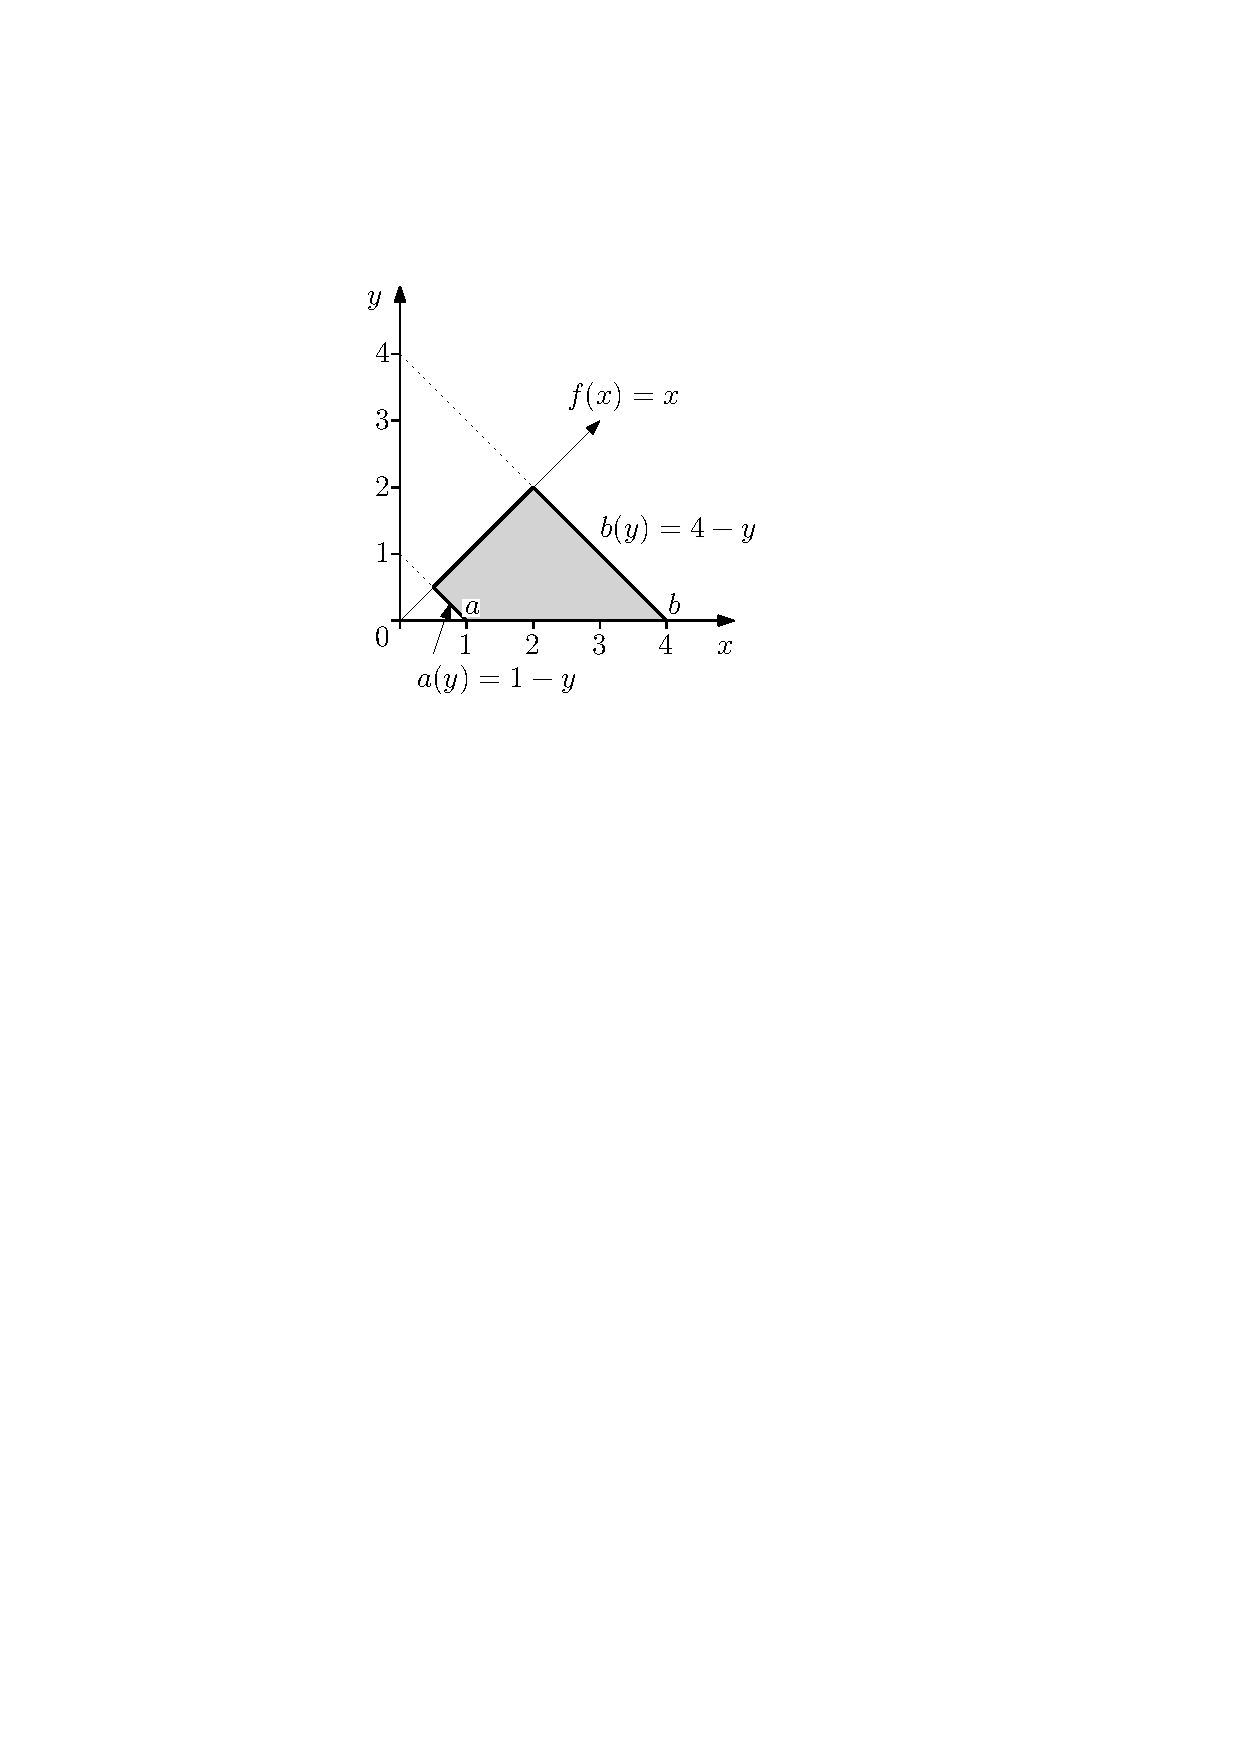
\includegraphics[width=0.3\textwidth]{fig12}
%\caption{Region bounded by the $x$-axis and the lines $f(x)=x$, $a(y)=1-y$, and $b(y)=4-y$. Reproduced from Quaestiones Mathematicae (2012) 35: 265-296 with permission \copyright~ NISC (Pty) Ltd.}
%\label{fig:ex1}
%\end{figure}
\begin{figure}[htb]
\centering
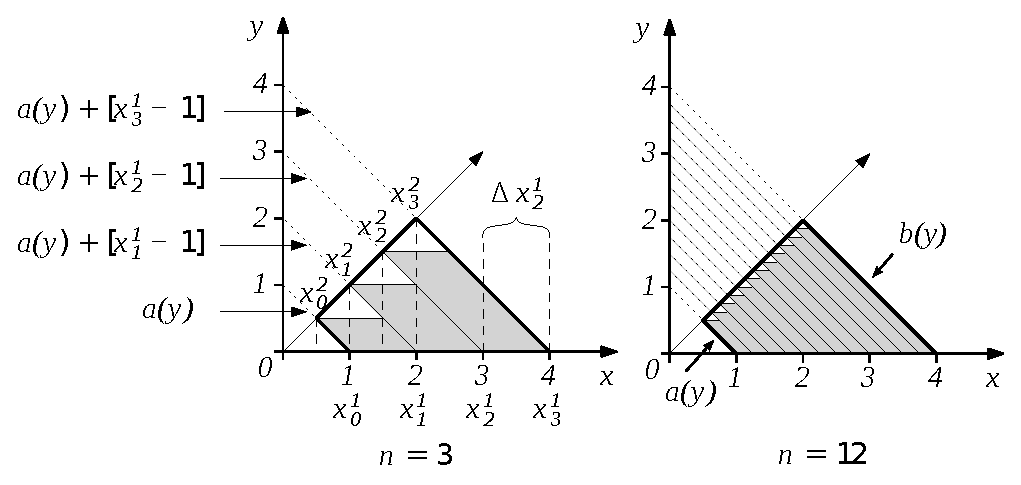
\includegraphics[width=0.75\textwidth]{fig13.eps}
\caption{Region bounded by the $x$-axis and the lines $f(x)=x$, $a(y)=1-y$, and $b(y)=4-y$. The figure also depicts the partition points $x_i^2$ as used in the Cavalieri sum (see Eq.~\ref{eq:cav_sum}). Reproduced from Quaestiones Mathematicae (2012) 35: 265-296 with permission \copyright~ NISC (Pty) Ltd.}
\label{fig:caval2}
\end{figure}

\noindent
The area of $R$ can be determined as follows if we employ the classical notion of integration:
\begin{equation}
\int_0^2x\, dx+\int_2^44-x\, dx- \int_0^{\frac{1}{2}}x\, dx-\int_{\frac{1}{2}}^11-x\, dx = 3.75. 
\end{equation}

There, however, exists a more straightforward way do determine the area of $R$, i.e. we can sum together the area of non-rectangular integration strips inscribing $R$ instead of
rectangular strips. Moreover, the shape of these non-rectangular integration strips should be determined by the function $a(y)$. We can express this notion more formally as 
follows, let $(x_i^1)_{i=0}^{n}$ denote a partition on the $x$-axis, such that $a = x_0^1 < x_1^1 < \cdots < x_n^1 = b$, and $\Delta x_i^1 = x_{i+1}^1 - x_i^1$.
We are now able to construct the following sum (the lower Cavalieri sum):
\begin{equation}
\label{eq:cav_sum}
\sum_{i=0}^{n-1} f(x_i^2)\Delta x_i^1.
\end{equation}
The partition points $(x_i^2)_{i=0}^{n}$ are depicted in Fig.~\ref{fig:caval2}. Note that Equation~\ref{eq:cav_sum} approximates the area of $R$. In the limit Equation~\ref{eq:cav_sum} approaches 
the Cavalieri integral:
\begin{equation}
\label{eq:caval1}
\int_{a(y)}^{b(y)}f(x)\, dx = \lim_{n\to \infty}\sum_{i=0}^{n-1} f(x_i^2)\Delta x_i^1.
\end{equation}
It is, however, quite hard to evaluate the above integral directly. Fortunately, it is easy to convert a Cavalieri integral into an equivalent Riemann or Riemann-Stieltjes 
integral using the transformation functions $h$ and $g$. Expressed mathematically:
\begin{equation}
 x
\end{equation}




\noindent
Instead of trying to determine the area of $R$ using rectangular integration strips, it seems more natural 
to use integration strips whose sides are translations of $a(y)$. Cavalieri's principle tells us that the area of an 
arbitrary shaped integration strip is the product of its height and the length of its base. The area of $R$ 
can be approximated by summing together multiple non--rectangular integration strips that inscribe $R$. This concept is illustrated in Fig.~\eqref{fig:caval2}. 
More formally, consider a partition $(x_i^1)_{i=0}^{n}$ on the $x$-axis, such that $a = x_0^1 < x_1^1 < \cdots < x_n^1 = b$, and $\Delta x_i^1 = x_{i+1}^1 - x_i^1$.
%As Fig.~\ref{fig:caval2} illustrates, the partition points $x_i^1$ are chosen to coincide with the $x$-coordinates at which the sides of the 
%integration strips intersect the $x$-axis. Fig.~\ref{fig:caval2} also shows us that another partition $(x_i^2)_{i=0}^{n}$, on the $x$-axis, such that $a' = x_0^2 < x_1^2 < \cdots < x_n^2 = b'$
%is automatically created when we make use of non--rectangular integration strips. The partition points $x_i^2$ 
%coincide with the $x$-coordinates at which the sides of the 
%integration strips intersect $f(x)$. 
Let us now construct the following sum (i.e. a lower Cavalieri sum) with which we can approximate the area 
of $R$:
\begin{equation}
\label{eq:cav_sum}
\sum_{i=0}^{n-1} f(x_i^2)\Delta x_i^1.
\end{equation}
The partition points $(x_i^2)_{i=0}^{n}$ are depicted in Fig.~\ref{fig:caval2}.
The above sum can be interpreted as summing together the areas associated with $n$ non--rectangular integration strips.
The left panel of Fig.~\ref{fig:caval2} depicts the scenario in which we made use of three integration strips.  
The right panel of Fig.~\ref{fig:caval2} illustrates that the larger $n$ becomes the better Eq.~\eqref{eq:cav_sum} approximates the area of $R$. In the limit Eq.~\eqref{eq:cav_sum} approaches the Cavalieri integral:
\begin{equation}
\label{eq:caval1}
\int_{a(y)}^{b(y)}f(x)\, dx = \lim_{n\to \infty}\sum_{i=0}^{n-1} f(x_i^2)\Delta x_i^1.
\end{equation}

\noindent
It is however hard to evaluate Eq.~\eqref{eq:caval1} in its present form. Fortuitously, we can transform the Cavalieri sum given in Eq.~\eqref{eq:caval1} into an ordinary Riemann sum
if we can determine an expression for $x_i^2$ in terms of the partition points $x_i^1$, for all $i=0,1,\ldots,n$. Consider the collection of functions $\{a(y) + [x_i^1-a] = x_i^2: i=0,1,\ldots,n\}$. To find the partition points $x_i^2$ in terms of $x_i^1$ we substitute the function $f(x_i^2)$ for $y$ to obtain:
\begin{align*}
a\circ f (x_i^2)+[x_i^1-1] &= x_i^2\\
x_i^2 &= \dfrac{x_i^1}{2},
\end{align*}
so that we have the general expression $x_i^2=h(x_i^1)$, with $h(x)=x/2$.\\

\noindent
The function $h$ allows us to rewrite the Cavalieri integral as an equivalent Riemann integral:
\begin{equation}
\label{eq:h_int}
\lim_{n\to \infty}\sum_{i=0}^{n-1} f(x_i^2)\Delta x_i^1 =  \lim_{n\to \infty}\sum_{i=0}^{n-1} f \circ h (x_i^1)\Delta x_i^1 = \int_a^b f \circ h (x)\, dx.
\end{equation}

\noindent
It is now possible to compute the Cavalieri integral by evaluating its equivalent Riemann integral:
\begin{equation}
\int_{a(y)}^{b(y)}f(x)\, dx = \int_a^b f \circ h (x)\, dx = \dfrac{1}{2}\int_1^4x\, dx = 3.75.  
\end{equation}

\noindent
Interestingly, the function $g=h^{-1}$ allows us to rewrite the Cavalieri integral as an equivalent Riemann--Stieltjes integral:
\begin{equation}
\label{eq:g_int}
\lim_{n\to \infty}\sum_{i=0}^{n-1} f(x_i^2)\Delta x_i^1 =  \lim_{n\to \infty} \sum_{i=0}^{n-1} f(x_i^2)[g(x_{i+1}^2)-g(x_{i}^2)] = \int_{a'}^{b'} f \, dg(x). 
\end{equation}

\noindent
We can therefore also compute the Cavalieri integral by evaluating its equivalent Riemann--Stieltjes integral:
\begin{equation}
\int_{a(y)}^{b(y)}f(x)\, dx = \int_{a'}^{b'} f \, dg(x) = \int_{\frac{1}{2}}^2x\, d2x = 3.75.  
\end{equation}

\noindent
We can quickly verify this to be correct by evaluating the area of $R$ with ordinary Riemann integration:
\begin{equation}
\int_0^2x\, dx+\int_2^44-x\, dx- \int_0^{\frac{1}{2}}x\, dx-\int_{\frac{1}{2}}^11-x\, dx = 3.75. 
\end{equation}


\section{Riemann-Liouville Fractional Integral}
Let
\begin{equation}
If(x) := \int_0^x f(t) dt.
\end{equation}
If we apply the above operator in a repetative manner to $f$ we obtain the $n$th antiderivative of $f$ based at 0:
\begin{equation}
\label{eq:n_anti}
I^nf(x) = \int_0^x\int_0^{x_1}\cdots \int_0^{x_{n-1}}f(x_n)~dx_n\cdots dx_2 dx_1.
\end{equation}
Applying Cauchy's formula for repetative integration to the above $n$th antiderivative of $f$ helps us express the above $n$th antiderivative as a single integral. 
Applying Cauchy's formula to Equation~\ref{eq:n_anti} results in:
\begin{equation}
\label{eq:cauchy}
I^nf(x) = \frac{1}{(n-1)!}\int_0^x (x-t)^{n-1}f(t)~dt.
\end{equation}
As an example if $f(x)=x$ and $n=2$ then Equation~\ref{eq:cauchy} reduces to:
\begin{equation}
I^2f(x) = \int_0^x (x-t)t~dt = \frac{t^2x}{2} - \frac{t^3}{3} \Bigg |_0^x = \frac{x^3}{3!}.
\end{equation}
The definition in Equation~\ref{eq:cauchy} can now be extended to an arbitrary fractional order by replacing $(n-1)!$ with the Gamma function:
\begin{equation}
\label{eq:frac_integral}
I^{\alpha}f(x) = \frac{1}{\Gamma(\alpha)}\int_0^x (x-t)^{\alpha-1}f(t)~dt.
\end{equation}
Equation~\ref{eq:frac_integral} is known as the Riemann-Liouville fractional integral of order $\alpha$. As an example if $f(x)=x$ and $\alpha=\frac{1}{2}$ then 
Equation~\ref{eq:frac_integral} reduces to:
\begin{equation}
I^{\frac{1}{2}}f(x) = \frac{1}{\Gamma(\frac{1}{2})} \int_0^x \frac{t}{\sqrt{x-t}} dt = \frac{1}{\sqrt{\pi}}\left [ -\frac{2}{3}\sqrt{x-t}(t+2x)\right] \Bigg |_0^x=\frac{4}{3\sqrt{\pi}}x^{\frac{3}{2}}. 
\end{equation}
Furthermore, it is straightforward to show that the $I$ operator satisfies:
\begin{equation}
I^{\alpha}I^{\beta}f(x) = I^{\alpha+\beta}f(x). 
\end{equation}

\section{Geometric Interpretation of Fractional Integrals}

The fractional integral is defined as (need to be more explicit here). Need to add how it has come about... Start with a single integral, expand to the general case and then 
to a general $\alpha$. 
\begin{equation}
\frac{1}{\Gamma(\alpha)}\int_{0}^{t}f(\tau)(t-\tau)^{\alpha-1}~d\tau
\end{equation}

Podlubny showed that the fractional integral can be rewritten as a Riemann-Stieltjes integral:
\begin{equation}
\label{eq:rs}
\int_0^{t} f(\tau)~dg_t(\tau),
\end{equation}
with 
\begin{equation}
g_t^{\alpha}(\tau) = \frac{\left \{t^{\alpha} - (t-\tau)^{\alpha} \right \}}{\Gamma(\alpha+1)}. 
\end{equation}

We can now transform Equation~\ref{eq:rs} into an equivalent Cavalieri integral:
\begin{equation}
\label{eq:cav}
\int_{a_t^{\alpha}(y)}^{b_t^{\alpha}(y)} f(\tau)~d\tau, 
\end{equation}
with
\begin{equation}
a_t^{\alpha}(y) = f^{-1}(y) - \frac{t^{\alpha}-(t-f^{-1}(y))^{\alpha}}{\Gamma(\alpha+1)}
\end{equation}

Since Equation~\ref{eq:cav} is a Cavalieri integral, it has a clear geometric interpretation. The integral in eq xxx can be interpreted as an infinite
sum of infinitesimally small non–rectangular integration strips whose shape is determined by $\alpha$ and $t$. The shape of the integration 
strip will change if either $\alpha$ or $t$ is changed. If $\alpha$ is equal to one, however, then the integral 
reduces to a normal Riemann integral as the integration strips become rectangular for this particular choice of $\alpha$ (its shape is now also no longer affected by $t$).








\section{First-level section heading}

Section headings use an initial capital letter on the first word, with subsequent words lowercase.  In general, the style of the journal is to leave all section headings unnumbered.  Consult the journal editor if you wish to depart from this and other conventions.

\subsection{Second-level heading}

The same goes for second-level headings.  It is not necessary to add font commands to make the math within heads bold and sans serif; this change will occur automatically when the production style is applied.

\section{Graphics}

Figures for the \textsc{Journal} can be submitted as either color or black \& white graphics.  Generally, color graphics will be used for the online publication, and converted to black \& white images for the print journal.  We recommend using whatever graphics program you are most comfortable with, so long as the submitted graphic is provided as a separate file using a standard file format.

For best results, please follow the following guidelines:
\begin{enumerate}
\item Bitmapped file formats---preferably TIFF or JPEG, but not BMP---are appropriate for photographs, using a resolution of at least 300 dpi at the final scaled size of the image.
\item Line art will reproduce best if provided in vector form, preferably EPS.
\item Alternatively, both photographs and line art can alternatively be provided as PDF files.  Note that creating a PDF does not affect whether the graphic is a bitmap or vector; saving a scanned piece of line art as PDF does not convert it to scalable line art.
\item If you generating graphics using a \TeX\ package, please be sure to provide a PDF of the manuscript.  In the production process, \TeX-generated graphics will eventually be converted to more conventional graphics so the \textsc{Journal} can be delivered in e-reader formats.
\item For photos of contributing authors, we prefer photos that are not cropped tight to the author's profile, so that production staff can crop the head shot to an equal height and width.  If possible, avoid photographs that have excess shadows or glare.
\end{enumerate}

\section{Theorems, definitions, proofs, and all that}

Following the defaults of the \texttt{amsthm} package, styling is provided for \texttt{theorem}, \texttt{definition}, and \texttt{remark} styles, although the latter two use the same styling.

\begin{theorem}[Pythagorean Theorem]
Theorems, lemmas, axioms, and the like are stylized using italicized text. These environments can be numbered or unnumbered, at the author's discretion.
\end{theorem}

\begin{proof}
Proofs set in roman (upright) text, and conclude with an ``end of proof'' (q.e.d.) symbol that is set automatically when you end the proof environment.  When the proof ends with an equation or other non-text element, you need to add \verb~\qedhere~ to the element to set the end of proof symbol; see the \texttt{amsthm} package documentation for more details.
\end{proof}

\begin{definition}[Secant Line]
Definitions, remarks, and notation are stylized as roman text.  They are typically unnumbered, but there are no hard-and-fast rules about numbering.
\end{definition}

\begin{remark}
Remarks stylize the same as definitions.
\end{remark}

Note that the \textit{College Mathematics Journal\/} is meant to be accessible to a broad audience, so heavy use of theorem-like formalisms is generally discouraged.

\begin{acknowledgment}
The authors wish to thank the Greek polymath Anonymous, whose prolific works are an endless source of inspiration.
\end{acknowledgment}

\begin{abstract}
An abstract should not contain concrete mathematics, but rather should be discrete.  Be brief and avoid using mathematical notation except where absolutely necessary, since this brief synopsis will be used by search engines to identify your article!
\end{abstract}

\begin{thebibliography}{1}
\bibitem{parker13} Adam Parker, Who solved the Bernoulli equation and how did they do it? \textit{Coll. Math. J.} \textbf{44} (2013) 89--97.

\bibitem{hopkins} Brian Hopkins, ed., \textit{Resources for Teaching Discrete Mathematics}, Mathematical Association of America, Washington DC, 2009.
\end{thebibliography}
\vfill\eject

\end{document}
